\documentclass[11pt,a4paper]{article}
\usepackage[T1]{fontenc}
\usepackage[utf8]{inputenc}
\usepackage{lmodern,microtype}
\usepackage[margin=26mm]{geometry}
\usepackage{amsmath,amssymb,bm,graphicx,booktabs,tabularx,authblk}
\usepackage[numbers,sort&compress]{natbib}
\renewcommand{\bibfont}{\small}
\setlength{\bibsep}{4pt plus 1pt minus 1pt}
\usepackage[colorlinks=true,linkcolor=blue,citecolor=blue,urlcolor=blue]{hyperref}
\hypersetup{pdftitle={From Bellissard's gap labeling to atomistic quasiperiodic bilayers},pdfauthor={Thomas D. Kühne, Vladislav Efremkin, Emil Prodan}}
\newcommand{\Tr}{\operatorname{Tr}}
\newcommand{\tr}{\operatorname{tr}}
\newcommand{\spec}{\operatorname{spec}}
\newcommand{\ii}{\mathrm{i}}
\newcommand{\dd}{\mathrm{d}}
\newcommand{\Id}{\mathbf{1}}
\setlength{\emergencystretch}{2em}
\setlength{\parskip}{0.25em}
\setlength{\parindent}{1.2em}
\renewcommand{\Authfont}{\large}
\renewcommand{\Affilfont}{\small}
\setlength{\affilsep}{0.7em}

\title{From Bellissard's gap labeling\\to atomistic quasiperiodic bilayers}
\author[1,2,3]{Thomas D. K\"uhne\thanks{Corresponding author: \href{mailto:tkuehne@cp2k.org}{tkuehne@cp2k.org}}}
\author[1,2]{Vladislav Efremkin}
\author[4]{Emil Prodan}
\affil[1]{Center for Advanced Systems Understanding (CASUS), Conrad-Schiedt-Stra{\ss}e 20, 02826 G\"orlitz, Germany}
\affil[2]{Helmholtz-Zentrum Dresden-Rossendorf (HZDR), Bautzner Landstra{\ss}e 400, 01328 Dresden, Germany}
\affil[3]{Institute of Artificial Intelligence, Technische Universit\"at Dresden, Helmholtzstra{\ss}e 10, 01069 Dresden, Germany}
\affil[4]{Department of Physics, Yeshiva University, New York, New York 10016, USA}
\date{}

\begin{document}
\maketitle
\begin{abstract}
Bellissard's formulation of solid-state physics replaces periodicity as the organizing principle by an algebra of covariant observables. This perspective provides a natural language for quasiperiodic bilayers, but its connection to atomistic electronic-structure calculations requires care. We explain the passage from a family of geometries to a bulk spectral projector, its integrated density of states, and the topological pairings that describe phason-dependent response. A finite honeycomb-bilayer model illustrates how interlayer coupling reorganizes spectral moments without, by itself, establishing a topological gap. We then distinguish a Hamiltonian operator from its nonorthogonal matrix representation, and a bulk state count from a layer-projected density of states. The resulting framework identifies which numerical observations are evidence for hybridization, which are necessary for gap labeling, and which additional calculations support a quantized response. The aim is a practical connection between Bellissard's mathematical viewpoint and atomistic modeling, rather than a new claim of a topological phase in a specific material.
\end{abstract}

\section{Bellissard's viewpoint beyond periodic crystals}

Bloch theory organizes the electronic structure of a periodic crystal through a family of finite matrices over the Brillouin zone. Quasiperiodic structures retain reproducible local environments without possessing a common translation cell. The loss of a Brillouin zone does not, however, imply the loss of a bulk description or of quantized observables. A central contribution of Bellissard was to formulate these questions in terms of an algebra of physical observables and its $K$-theory~\cite{bellissard1986}. The noncommutative treatment of the quantum Hall effect~\cite{bellissard1994} and subsequent gap-labeling results for aperiodic patterns~\cite{bellissard2006} show why this shift is more than a replacement of notation.

The key object is not an isolated finite Hamiltonian matrix. It is a covariant family of operators, together with a prescription for bulk averaging. A spectral gap then defines a projection in the observable algebra. Its class can be paired with a trace to count states and, with additional structure, with Chern cocycles to describe transport. These pairings answer related but distinct questions. In particular, a recognizable spectral pattern is neither a state count nor a measurement of a topological response.

Quasiperiodic photonic and acoustic systems make this distinction concrete. Phason-dependent pumping and boundary modes provide information beyond the density of states~\cite{kraus2012,ni2019}. Twisted mechanical structures extend this connection to geometric incommensurability in two dimensions~\cite{rosa2021}. Electronic bilayers introduce further ingredients, including multiple orbitals, self-consistency, structural relaxation, and nonorthogonal basis functions. Their analysis benefits from keeping the same mathematical questions visible throughout the modeling chain.

This article develops that connection in three stages. We first identify the bulk objects entering gap labeling and distinguish phasons from changes of twist angle. We then use finite bilayer model calculations to separate coupling-induced spectral reconstruction from topology. Finally, we translate the operator formulation into quantities accessible to atomistic electronic-structure codes. The discussion builds on established theory and includes an illustrative model analysis, but no first-principles materials results.

\section{From a family of patterns to a bulk state count}
\label{sec:bulk}

\subsection{Covariance and the trace}

Consider first a lattice description with $q$ orthonormal internal orbitals per reference cell. Let $\Omega$ be a compact space of patterns with a translation action $T_{\bm n}$, $\bm n\in\mathbb Z^2$. A family of bounded, self-adjoint Hamiltonians $\hat H_\omega$ on $\ell^2(\mathbb Z^2)\otimes\mathbb C^q$ is covariant if
\begin{equation}
 U_{\bm n}\hat H_\omega U_{\bm n}^{-1}=\hat H_{T_{\bm n}\omega}.
 \label{eq:covariance}
\end{equation}
Locality, continuity in the pattern, and covariance specify the observable algebra $\mathcal A$. Finite-range or sufficiently decaying hopping is a useful setting for this construction. The translation convention in Eq.~\eqref{eq:covariance} fixes the corresponding convention for the action on patterns.

For an invariant ergodic probability measure $\mu$ on $\Omega$, the bulk trace is
\begin{equation}
 \tau(A)=\int_\Omega \tr_q\langle\bm 0|A_\omega|\bm 0\rangle\,\dd\mu(\omega)
 =\lim_{R\to\infty}\frac{\Tr(\chi_R A_\omega\chi_R)}{|\Lambda_R|}.
 \label{eq:trace}
\end{equation}
Here $\chi_R$ selects expanding square reference-cell regions $\Lambda_R$, whose boundary-to-volume ratio vanishes. Under the stated ergodic assumptions the limit holds for almost every pattern, and $\tau(\Id)=q$. The normalization is states per reference cell, not states per plotted DOS peak. Unique ergodicity can strengthen the independence from the chosen pattern under the appropriate continuity assumptions.

Equation~\eqref{eq:trace} is a transparent lattice example, not a universal identification of a multilayer atomic structure with $\mathbb Z^2$. In a bilayer with independently varying site sets, an appropriate configuration-space or groupoid description may be required. A trace per physical area then has units of inverse area. General aperiodic frameworks address precisely the absence of a canonical global lattice indexing~\cite{bourne2018}. The choice of algebra and the normalization of its trace must precede a numerical assignment of gap labels.

\subsection{The projector and its label}

Suppose $E$ lies in a common spectral gap of the bulk family. Functional calculus gives a spectral projection
\begin{equation}
 P_E=\Id_{(-\infty,E]}(\hat H),\qquad P_E^2=P_E=P_E^*,\qquad
 \mathcal N(E)=\tau(P_E).
 \label{eq:ids}
\end{equation}
The integrated density of states (IDS), $\mathcal N(E)$, is constant as $E$ moves within the gap. Because the discontinuity of the indicator function lies outside the spectrum, $P_E$ belongs to the observable algebra. It defines a class in $K_0(\mathcal A)$, and the trace induces the homomorphism
\begin{equation}
 \tau_*:K_0(\mathcal A)\longrightarrow\mathbb R,
 \qquad [P]\longmapsto\tau(P).
 \label{eq:kzero}
\end{equation}
Bellissard's gap-labeling viewpoint constrains the possible values of the IDS through the range of this map~\cite{bellissard1986,bellissard2006}. It does not assert that every permitted label corresponds to an open gap. Nor is the trace pairing generally injective. Distinct topological classes can share a state count, so the IDS need not determine all response coefficients.

A familiar illustration is the one-dimensional quasiperiodic Harper family
\begin{equation}
 (\hat H_\phi\psi)_n=t(\psi_{n+1}+\psi_{n-1})
 +V\cos(2\pi\alpha n+\phi)\psi_n,
 \label{eq:harper}
\end{equation}
with irrational $\alpha$ and one orbital per site. For an actual spectral gap, the trace range gives
\begin{equation}
 \mathcal N(E)=m+n\alpha\in[0,1],\qquad m,n\in\mathbb Z.
 \label{eq:harperlabel}
\end{equation}
The spectral organization is closely related to the magnetic problem underlying the Hofstadter butterfly~\cite{hofstadter1976}. For a rational approximant $\alpha=p/q$ and a gap above $r$ bands, the corresponding counting relation is $r=mq+np$. One such rational equation alone does not uniquely determine an integer pair. Continuation across the family or an independent topological calculation supplies information that an isolated finite spectrum lacks. The sign relating $n$ to a pumping convention also depends on the orientation chosen for the phason cycle.

\section{Phasons, twist, and the meaning of a response}

At fixed twist angle and layer separation, a rigid relative displacement of two ideal infinite layers changes their registry. Observed from one reference layer, the displacement modulo the other layer's lattice provides two phason coordinates. In an incommensurate setting, reference-layer translations can sample this phason torus densely. This geometric construction motivates a covariant description, but the Hamiltonian's orbital content, relaxation rule, and locality still have to respect it.

A phason cycle varies registry within a specified family. Changing the twist angle generally changes the translation action itself, while changing separation changes the strength and range of interlayer coupling. These are useful controls but are not interchangeable coordinates. In particular, an angle-dependent DOS image is not an adiabatic pumping experiment.

The distinction is explicit for a periodic approximant to a one-dimensional pump. Let $P(k,\phi)$ be a smooth occupied-band projector, gapped on the full two-torus of dimensionless $k$ and $\phi$, both of period $2\pi$. With a fixed orientation, its first Chern number is
\begin{equation}
 C=\frac{\ii}{2\pi}\int_0^{2\pi}\!\dd k\int_0^{2\pi}\!\dd\phi\,
 \tr\!\left(P[\partial_kP,\partial_\phi P]\right)\in\mathbb Z.
 \label{eq:pump}
\end{equation}
For a filled, noninteracting band subspace in the adiabatic limit, this integer determines transported particle number, with the sign set by the orientation and current convention~\cite{thouless1983}. Quasiperiodic systems implement related synthetic-dimensional responses~\cite{kraus2012,prodan2015}, and sliding moir\'e patterns provide bilayer examples~\cite{su2020,fujimoto2020}.

For suitable two-dimensional twisted models, spatial translations and two phason coordinates lead to a higher-dimensional noncommutative algebra~\cite{rosa2021}. This is a statement about the model's covariance structure, not an automatic consequence of having two atomic sheets. Extensions of gap labeling to multilayers likewise depend on the specified effective description~\cite{yoshii2023}. A response involving a spatial direction and a phason must also be distinguished from an ordinary Hall response involving two physical spatial directions. A real, time-reversal-symmetric model may have vanishing ordinary Hall conductivity while allowing a nontrivial mixed spatial-phason pump.

The spectral-gap setting is deliberately the starting point here. Quantization can also survive in a mobility gap, under suitable localization and regularity conditions~\cite{bellissard1994,bourne2018}. A mobility gap is not an interval of necessarily vanishing DOS. Inferring it requires localization information that a dark region in a broadened spectrum cannot provide.

\section{What a finite bilayer model can establish}
\label{sec:model}

\subsection{A geometric coupling parameter}

Consider two identical honeycomb disks. With nearest-neighbor distance $a$, primitive vectors $\bm a_1=(\sqrt{3}a,0)$ and $\bm a_2=(\sqrt{3}a/2,3a/2)$, and basis positions $(0,0)$ and $(0,a)$, retain the $N$ sites inside radius $R$. Place one disk at height zero and the other, rotated by $\theta$, at height $d$. On orthonormal site states define
\begin{equation}
 \hat H_{\mathrm{TB}}=\sum_{i\ne j}t_0\exp(-r_{ij}/\xi)|i\rangle\langle j|,
 \qquad t_0>0,\quad \xi>0.
 \label{eq:bilayer}
\end{equation}
All pairs are included, the on-site term is zero, and $r_{ij}$ is the three-dimensional distance. This is an isotropic geometric model. It is not an orbital-resolved parametrization of graphene and does not resolve the angular dependence of carbon bonding.

The nearest-neighbor intralayer hopping $t_{\mathrm{nn}}=t_0\exp(-a/\xi)$ provides an exact energy scale. The matrix of $\hat h=\hat H_{\mathrm{TB}}/t_{\mathrm{nn}}$ is
\begin{equation}
 \bm h=\begin{pmatrix}\bm D&\bm B\\\bm B^\dagger&\bm D\end{pmatrix},
 \quad D_{ij}=(1-\delta_{ij})e^{(a-|\bm r_i-\bm r_j|)/\xi},
 \quad B_{ij}=e^{(a-\sqrt{|\bm r_i-\mathsf R_\theta\bm r_j|^2+d^2})/\xi}.
 \label{eq:block}
\end{equation}
The matrices are representations in the specified finite site basis, whereas $\hat h$ denotes the operator. The largest possible interlayer-to-intralayer hopping ratio is
\begin{equation}
 \frac{t_\perp^{\max}}{t_{\mathrm{nn}}}=e^{(a-d)/\xi}.
 \label{eq:coupling}
\end{equation}
It is attained by vertically aligned sites, not by every pair. Thus a small change of $d$ relative to the decay length $\xi$ can substantially alter hybridization. For $\xi/a=0.03$ and $d/a=0.99,0.98,0.97$, this ratio is approximately $1.40,1.95,2.72$. These dimensionless separations have no prescribed conversion to a first-principles interlayer distance.

\subsection{A trace identity and its numerical illustration}

The normalized second spectral moment of the finite matrix is
\begin{equation}
 \mu_2=\frac{1}{2N}\sum_{\nu=1}^{2N}\epsilon_\nu^2
 =\frac{\Tr\bm h^2}{2N}
 =\underbrace{\frac{\Tr\bm D^2}{N}}_{\text{intralayer}}
 +\underbrace{\frac{\|\bm B\|_F^2}{N}}_{\text{interlayer}},
 \label{eq:moment}
\end{equation}
where $\epsilon_\nu$ are dimensionless eigenvalues and $\|\cdot\|_F$ is the Frobenius norm. The first moment vanishes because the diagonal of $\bm h$ is zero, so $\mu_2$ is also its spectral variance. Equation~\eqref{eq:moment} is an exact matrix identity. It isolates the added spectral variance due to interlayer coupling without requiring a visual interpretation of a DOS map.

\begin{figure}[tbp]
 \centering
 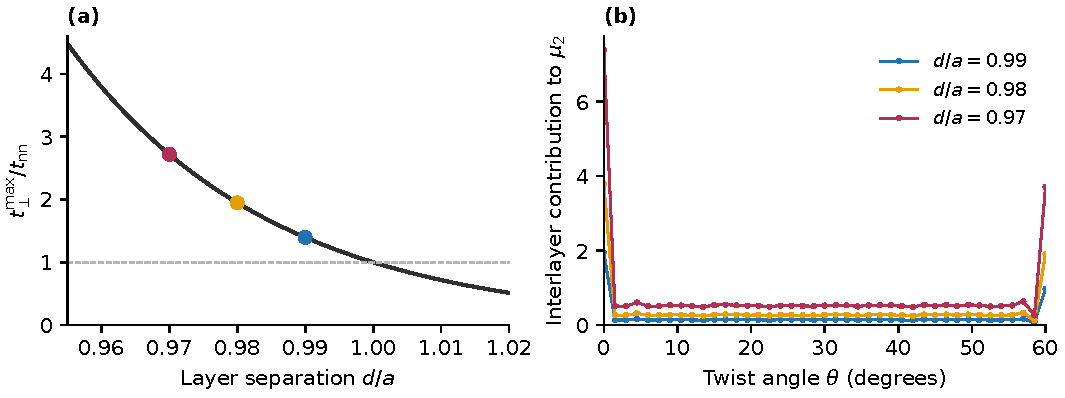
\includegraphics[width=\textwidth]{figures/bellissard_model_moments.pdf}
 \caption{Geometric coupling and a finite spectral trace. (a) The maximum interlayer hopping relative to nearest-neighbor intralayer hopping, Eq.~\eqref{eq:coupling}, for $\xi/a=0.03$. Colored points mark the three calculated separations. (b) The interlayer contribution $\|\bm B\|_F^2/N$ to the second spectral moment for open honeycomb disks with $R/a=25$ and $N=1510$ sites per layer. Each curve contains 41 directly evaluated angles from $0^\circ$ to $60^\circ$. Lines connect samples and do not resolve narrower angular structures. The same quantity is independently recovered from all 3020 eigenvalues using Eq.~\eqref{eq:moment}. No DOS broadening, gap assignment, or topological invariant enters this figure.}
 \label{fig:moments}
\end{figure}

Figure~\ref{fig:moments} evaluates this decomposition for $R/a=25$ and $\xi/a=0.03$. The intralayer contribution is identical for all angles and separations. The interlayer contribution depends on registry as well as separation, and increases when $d$ is reduced at fixed angle because every entry of $\bm B$ increases. Direct sums of squared hoppings and second moments of the archived eigenvalues agree to an absolute tolerance of $10^{-10}$ across all 123 spectra. This check tests the trace normalization and the spectral calculation, not a thermodynamic limit.

The relation to Bellissard's viewpoint is the distinction between a finite normalized trace and a bulk trace on a specified algebra. A second moment averages a polynomial of the Hamiltonian. Gap labeling instead concerns the trace of a spectral projection, whose existence as a stable bulk object requires a gap. A growing $\mu_2$ establishes a growing spectral variance but does not imply a new gap, a fractal spectrum, or a nonzero Chern number. Even fully converged spectral moments would not replace the projector and response calculations in Eqs.~\eqref{eq:ids} and~\eqref{eq:pump}.

The disk geometry makes the finite calculation reproducible and treats the two layers symmetrically. It does not eliminate boundaries. Registry-sensitive peaks in Fig.~\ref{fig:moments} should therefore not be interpreted as bulk singularities without a size and angular-resolution study. Nor does equality of two DOS maps establish equality of their projectors, since the eigenvectors contain information that the DOS discards.

\section{From nonorthogonal matrices to physical observables}

\subsection{A change of representation is not a change of Hamiltonian}

Atom-centered basis functions $\{|\chi_\mu\rangle\}$ generally overlap. A finite-basis electronic-structure calculation solves
\begin{equation}
 \bm H\bm c_n=\varepsilon_n\bm S\bm c_n,
 \qquad H_{\mu\nu}=\langle\chi_\mu|\hat H|\chi_\nu\rangle,
 \qquad S_{\mu\nu}=\langle\chi_\mu|\chi_\nu\rangle.
 \label{eq:generalized}
\end{equation}
For a linearly independent basis, $\bm S$ is positive definite. Symmetric orthogonalization gives~\cite{lowdin1950}
\begin{equation}
 \widetilde{\bm H}=\bm S^{-1/2}\bm H\bm S^{-1/2},
 \qquad \widetilde{\bm c}_n=\bm S^{1/2}\bm c_n,
 \qquad \widetilde{\bm c}_n^\dagger\widetilde{\bm c}_m=\delta_{nm}.
 \label{eq:lowdin}
\end{equation}
This represents the same projected operator in an orthonormal basis. Diagonalizing $\bm H$ as though $\bm S=\bm I$ would instead solve a different problem. Near-linear dependencies must be controlled before taking inverse square roots. An overlap-eigenvalue cutoff changes the retained subspace and must be documented.

For a sharp energy cutoff in a finite-system gap, the orthonormal-coordinate projector is
\begin{equation}
 \widetilde{\bm P}_E=\sum_{\varepsilon_n\leq E}
 \widetilde{\bm c}_n\widetilde{\bm c}_n^\dagger.
 \label{eq:finiteprojector}
\end{equation}
Its ordinary matrix trace counts occupied one-particle states in that finite basis. Passing from this count to a bulk IDS still requires a controlled sequence of geometries and a fixed physical normalization. Adding Gaussian basis functions should not silently change the definition of states per cell or per area.

\subsection{Why a projected DOS is not a gap label}

Let $\bm Q_L$ be an orthogonal projector onto selected L\"owdin orbitals. The projected DOS, before broadening, is
\begin{equation}
 \rho_L(E)=\sum_n w_n^{(L)}\delta(E-\varepsilon_n),
 \qquad w_n^{(L)}=\widetilde{\bm c}_n^\dagger\bm Q_L\widetilde{\bm c}_n.
 \label{eq:projecteddos}
\end{equation}
Unlike the total state count, these weights may be fractional. If a set of mutually orthogonal orbital projectors sums to the identity, summing their DOS recovers the total DOS for the same eigenstates and normalization. A different population-analysis convention need not assign the same layer weights.

A two-level example already exposes the logical limitation. For $\widetilde{\bm H}=\operatorname{diag}(\varepsilon_a,\varepsilon_b)$ and $\bm Q_L=\operatorname{diag}(1,0)$, the projected DOS has no weight at $\varepsilon_b$, although the full Hamiltonian has an eigenstate there. More generally, $\bm Q_L\widetilde{\bm P}_E\bm Q_L$ is not a projection unless the relevant subspaces commute. Its weighted trace therefore does not inherit the interpretation of a $K_0$ gap label. A layer-resolved depletion is a useful diagnostic of orbital character, not proof of a bulk spectral gap.

Display broadening and electronic occupations require a separate distinction. Convolution with a kernel of width $\eta$ smooths spectral data and can hide small gaps. Fermi--Dirac smearing changes occupations. At nonzero temperature the matrix $f_\beta(\widetilde{\bm H})$ is generally not idempotent and is not the sharp projector appearing in Eq.~\eqref{eq:ids}. Neither operation supplies a topological classification by itself.

\subsection{Parameter-dependent bases and Berry geometry}

Orthogonalization at a fixed geometry is insufficient for a phason derivative if the basis itself moves. Write $B(\lambda)=\chi(\lambda)\bm S(\lambda)^{-1/2}$ for the map from orthonormal coordinates to physical states, with $B^\dagger B=\bm I$. On a local parameter patch, let $\widetilde{\bm C}(\lambda)$ contain a smooth occupied orthonormal-coordinate frame. The physical occupied frame is $\Psi=B\widetilde{\bm C}$, and its Berry connection is
\begin{equation}
 \mathcal A_\lambda=\ii\Psi^\dagger\partial_\lambda\Psi
 =\ii\widetilde{\bm C}^\dagger\partial_\lambda\widetilde{\bm C}
 +\ii\widetilde{\bm C}^\dagger B^\dagger(\partial_\lambda B)\widetilde{\bm C}.
 \label{eq:basisconnection}
\end{equation}
The second term accounts for basis motion. Omitting it is justified only when the chosen representation makes it vanish or when an equivalent covariant overlap construction already includes it. Discrete overlaps between physical states at neighboring geometries offer a practical route, provided the cross-geometry basis overlaps are treated consistently. A basis-invariant spectrum at every geometry does not, by itself, guarantee a basis-consistent Berry curvature across geometries.

Electronic-structure packages such as CP2K provide a route to atomistic Hamiltonians and state-resolved quantities~\cite{cp2k2020,cp2k2026}. The UZH protocol illustrates why basis-set and pseudopotential errors should be separated~\cite{uzh2026perspective}. These controls remain necessary when the target quantity is topological. They do not establish that the self-consistent effective Hamiltonian defines the required covariant, smoothly parameterized family. Consistent spin treatment, structural relaxation, and branch selection of the self-consistent solution are additional requirements. A Kohn--Sham spectral gap must also be distinguished from a many-body excitation gap.

\section{A hierarchy of evidence for atomistic gap labeling}

The mathematical stability statement provides a useful standard for numerical practice. Let $E$ lie a distance $\delta>0$ from the spectrum of a bounded self-adjoint $\hat H$ in a fixed observable algebra. If a self-adjoint perturbation $\Delta\hat H$ in that algebra satisfies $\|\Delta\hat H\|<\delta$, then
\begin{equation}
 \hat H_s=\hat H+s\Delta\hat H,\quad 0\leq s\leq1,
 \qquad \operatorname{dist}(E,\spec\hat H_s)
 \geq\delta-\|\Delta\hat H\|>0.
 \label{eq:stability}
\end{equation}
The spectral projectors form a continuous path and retain their $K_0$ class. The spectral bound follows from the resolvent estimate, or equivalently from the Neumann-series criterion for invertibility. This statement explains robustness but does not turn an observed finite gap into a bulk one. Comparisons between changing basis spaces need a common embedding before an operator-norm estimate has this meaning.

Table~\ref{tab:evidence} separates the principal observables. The order matters: assigning an integer before establishing the relevant bulk projector reverses the logic of gap labeling. Conversely, demanding a quantized response from a diagnostic model moment asks that observable to answer a question it was not designed to address.

\begin{table}[!ht]
 \centering
 \small
 \caption{Different numerical objects support different physical conclusions.}
 \label{tab:evidence}
 \begin{tabularx}{\textwidth}{@{}>{\raggedright\arraybackslash}p{0.23\textwidth}>{\raggedright\arraybackslash}X>{\raggedright\arraybackslash}X@{}}
 \toprule
 Object & Direct information & Additional requirement for topology \\
 \midrule
 Finite spectral moment & Averaged spectral scale and coupling contributions & A bulk limit and a gapped spectral projector \\
 \addlinespace
 Layer-projected DOS & Spectral weight in a chosen subspace & Total spectral information and a projection-independent gap test \\
 \addlinespace
 Bulk IDS plateau & State count in an established spectral gap & A justified trace range and, where needed, further topological pairings \\
 \addlinespace
 Phason-dependent projector & Geometry of occupied states across a family & A converged invariant and the assumptions connecting it to response \\
 \bottomrule
 \end{tabularx}
\end{table}

A practical analysis begins by specifying the family of infinite structures, its covariance, the retained orbitals, and the trace normalization. Finite patches or periodic approximants can then be chosen to approach that family, rather than being treated as its definition. For a two-dimensional open patch, boundary state counts typically grow with perimeter while bulk counts grow with area. Boundary weight can vanish in a normalized DOS and still encode physically important spectral flow. Interior projections are therefore useful for diagnosing bulk gaps, while boundary-resolved calculations answer a complementary question.

The next step is to converge the full spectral information with respect to size, approximant order, basis quality, and the relevant numerical cutoffs. Candidate gaps must be distinguished from missing calculations, insufficient energy resolution, and finite-size level spacings. A consistent energy reference is needed to follow the same gap across a parameter family. Aligning each spectrum independently to its own Fermi level can obscure that tracking.

Only after this stage should an IDS plateau be compared with the trace range of the chosen algebra. Its persistence should be checked along the appropriate gapped family. If a pumping or Hall interpretation is sought, one should compute the corresponding pairing of the projector with spatial and/or phason derivatives, using consistent parameter-dependent bases. Boundary spectral flow or an explicit adiabatic transport calculation then offers an independent test of the proposed response. These checks complement one another and cannot be replaced by a visual resemblance to the Hofstadter butterfly.

\section{Perspective}

Bellissard's work supplies an organizing principle that is especially useful at the boundary between ideal models and atomistic calculations: define the algebra of observables, identify the bulk trace, and only then ask which topological information a computed quantity carries. The finite bilayer calculation here illustrates the first diagnostic stage. Interlayer coupling contributes a precisely identifiable amount to the spectral variance, and this contribution changes with registry. It establishes a spectral mechanism, not a topological classification.

The further passage to atomistic quasiperiodic bilayers is demanding but well posed. Nonorthogonal basis sets require metric-aware projectors, moving atoms require basis-consistent parameter derivatives, and self-consistency requires a reproducible covariant branch of solutions. Relaxation can change the pattern space itself, so its effect is not always captured by adding a small perturbation to a fixed Hamiltonian. These are opportunities for a closer interaction between electronic-structure methods and noncommutative geometry rather than reasons to separate the subjects.

The most useful legacy of gap labeling for this program is thus not a visual template for spectra. It is a disciplined connection between geometry, state counting, and response. Keeping these three levels distinct makes it possible to use simple model calculations constructively while identifying exactly what a materials calculation must establish before a topological conclusion follows.

\paragraph{Acknowledgment.}
This perspective is dedicated to Jean Bellissard on the occasion of his eightieth birthday and to the continuing influence of his work on the mathematics and physics of aperiodic solids.

\paragraph{Data and code availability.}
The source of this article, the bilayer model code and eigenvalue files, the spectral-moment analysis, and its tabulated output are available in \url{https://github.com/DCM-Uni-Paderborn/Hofstadter-Butterfly}. The reproducible analysis for Fig.~\ref{fig:moments} is \texttt{analysis/bellissard\_model\_moments.py}. This article contains no first-principles calculation or first-principles data analysis.

\paragraph{Use of AI-assisted tools.}
AI-assisted tools were used in drafting the text and developing the analysis script.

\bibliographystyle{unsrtnat}
\bibliography{references,bellissard_references}
\end{document}
